%!TEX root = ../thesis.tex
\chapter{Introduction}
\label{introduction}

\hl{introduzione a significato di way of working (in SW)
	cercare articoli da blog per spiegare
	martin fowler		

fare tracking delle isssue / bug è diventato difficile / complesso
	molti tool open source che fanno anche documentazione e code review (altri aspetti)

l'evoluzione negli ultimi anni nelle aziende IT
	necessità di organizzazione delle azienda e la necessità di avere una gerarchia (o simil gerarchia)

ho sperimentato questo approccio in athonet, mostrata interessata all'utilizzo di un gestionale sw di tipo agile per la gestione dei processi di sviluppo sw interni

I have sperimented ... 
}

\section{Premise}
	This document is a report of the two month curricular internship done between June and July 2019 at Athonet under the supervision of Dr. Fabio Giust.
	It contains a description of the work that I have done and an introduction to Agile and Scrum software developing methodologies.\\
	%todo togliere se non serve
	%todo aggiungere footnote sito dilbert
	To introduce or to describe some of the arguments I will be using some comic strips of Dilbert, a character invented by Scott Adams.
	It satirically represents the problems that can be present in a small or big company of software development.
	\begin{figure}[H]
		\centering
		
\includegraphics[width=1\textwidth]{resources/Dissertate}\\
		\caption[Dilbert, \Quote{Plan A}]{Dilbert, \Quote{Plan A}, Monday June 06, 2011}
	\end{figure}
	\hl{Aggiungere come sono i riferimenti e come sono le parole a glossario}
	
\section{The company}
	Athonet is a telecommunication company headquartered nearby Vicenza.
	It stem from the idea that broadband networking should be easily available to people in rural areas and to companies that work in mission critical services or special environments like shipping, mining companies or even hospitals (safety critical).\\
	%todo officially it started senza was?
	%todo aggiungere footnote sito ericsson?
	Officially it was started in 2004, although a working prototype of their idea was already developed by the CEO and CTO that were working alongside in Ericsson at that time.
	%todo inserire citaizione Athonet.com
	\begin{figure}[H]
		\centering
		
\includegraphics[width=.7\textwidth]{resources/ath_logo}\\
		\caption[Athonet's logo]{Athonet's logo}
	\end{figure}
	Low latency communication, reliability and security are at the core of what Athonet provides.
	%todo spiegare significato di LTE prima di introdurlo
	Their main product is PriMo, a device that allows to create a dedicated core network, or enterprise LTE.
	\begin{figure}[H]
		\centering
		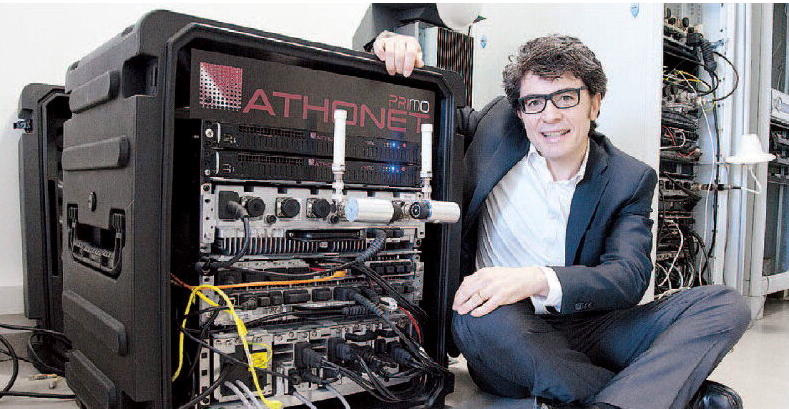
\includegraphics[width=.8\textwidth]{resources/gianluca_primo}\\
		\caption{The CTO, \textit{Gianluca Verin}, with Athonet's main product \textbf{\Quote{PriMo}}\cite{gianluca_primo}}
	\end{figure}
	In 2012, after a disastrous earthquake destroyed all the communication lines in Emilia Romagna, Athonet has reestablished connectivity, thus showing the how PriMo can be used on the field in emergency situations.\\
	Athonet installed PriMo at the top of a school, allowing them to cover the affected area not only for the operators of Servizio Civile but for the citizens as well.\\
	In December 2013, Athonet has been rewarded by Giorgio Napolitano, the then President of the Italian Republic, with a medal for merits for the sustainability in the digital sector.\\
	Lately they have migrated some of their functions to the cloud: by using AWS they have achieved a hybrid product, BubbleCloud, a plug and play solution that allows to locally deploy the physical Edge Nodes while managing them from the AWS cloud.\\
	This small business has much to offer, considering that some of it's competitors are giants like Nokia and Ericsson.\\
	As a proof of the continuous will to improve and for the solution it provides, Athonet has been awarded with four Global Mobile Awards at the GSMA Mobile World Congress, held in February 2019 in Barcelona.
	%todo inserire citazioni
%	https://www.millionaire.it/athonet-la-startup-italiana-che-trionfa-al-mobile-world-congress/#!
%	http://www.ilgiornale.it/news/interni/genio-torna-svezia-soffrire-nella-sua-italia-912407.html

\section{The project}
	It consists in installing and configuring two main software tools, Jira and Confluence, alongside plugins to add more functions and enhance their potentiality.
	However, the most important part of this project is not installing the software, but adapting it to the needs of the company.\\
	As said earlier Athonet my still be small, but it's a growing company, and because of this it needs to give itself some internal rules and specifications to follow when working on a task, communicating with the client or even share internal information to employees.
	Not only for themselves but for clients they work with as well, since most big companies require that their partners have internal regulations, no matter the number of people in the company.\\
	As I will explain in the following chapters Jira is an Issue Tracking System, a software that allows to follow the tasks (like resolving bugs or implementing features) that are related to a project, while Confluence is a software for sharing knowledge, that means sharing internal documents, keeping a wiki, having documentation available and even for customers.\\
	My task was to demonstrate that these tools are what Athonet needs to be a strong an coherent company, where information is always shared and available, while maintaining a history of changes, by creating an environment that suited their needs and that can evolve alongside the company.\\
	To do this I have learned the basics of Agile and Scrum methodologies, how a company operates internally and with their clients and how introducing a new tool may improve the way of working, even if it creates chaos at the beginning.

\section{Document organization}
	This thesis is organized as follows:
	\begin{itemize}
		\item Chapter 1 or \Quote{Introduction}: describes the overall content of this document
		\item Chapter 2 or \Quote{The internship project}: describes in detail the objectives and planning of the internship project
		\item Chapter 3 or \Quote{Agile processes and methodologies}: an introduction to the Agile software development
		\item Chapter 4 or \Quote{Jira and Confluence: the essentials}: describes the most valuable functionalities of Jira and Confluence
		\item Chapter 5 or \Quote{Project implementation}: details how the project has been implemented by dividing it into time periods
		\item Chapter 6 or \Quote{Conclusions}: contains the retrospective of the project, future developments and personal considerations
	\end{itemize}
